\subsection{Sigmoid Neuron}

While perceptrons are effectively step functions, flipping from $0$ to $1$, sigmoids are more smoothed out.
This means that a small change in the weight can lead to a small change in output.
The sigmoid function can be written as

\begin{align}
  \sigma = \frac{1}{1 + e^{-z}}
\end{align}

This means that a sigmoid neuron can be written as

\begin{align}
  \frac{1}{1 + e^{-\sum_i w_i x_i - b}}
\end{align}

where the $b$ stands for the bias of every input.
While this looks different than the perceptron at first glance it is just a more smoothed out version of it.
One key thing that we lose with the introduction of sigmoids is the linearity that perceptrons afforded us.
What we gain is the ability for our programs to automatically adjust their weights and biases because a small change in weights does lead to small change in output as shown in equation \ref{bias}.

\begin{align}\label{bias}
  \Delta y \approx \sum_i \frac{\partial y}{\partial w_i}\Delta w_i + \frac{\partial y}{\partial b}\Delta b
\end{align}

\begin{figure}[H]
  % https://blog.roboflow.com/activation-function-computer-vision/
  \centering
  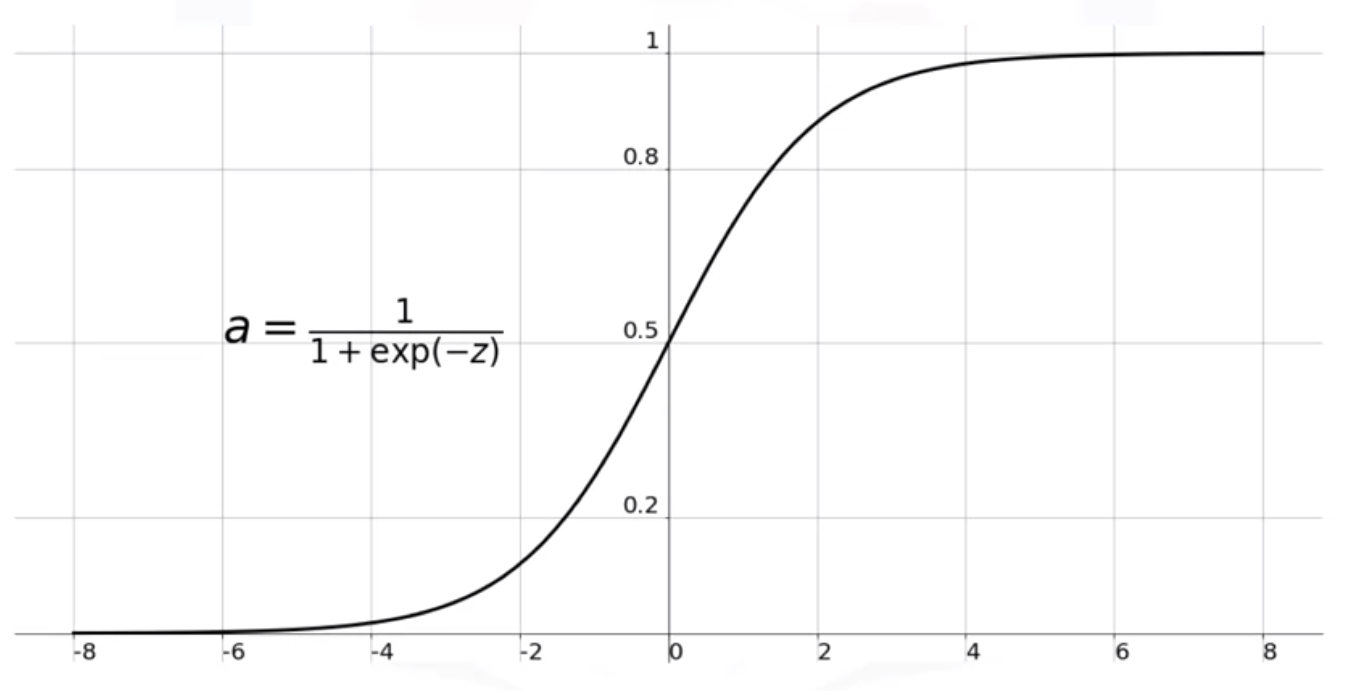
\includegraphics[width=80mm]{figures/sigmoid.png}
  \caption{Sigmoid Function}
  \label{network}
\end{figure}

More than the exact formula of the sigmoid neuron what matters is the shape.
As a result, other neurons can be used in it's stead which retain the property of having a small change in weight lead to a small change in output.
Some of the more popular of these functions (called activation functions) are RELU and softmax.
Each have their own advantages and disadvantages and may even be mixed in the same neural network

